While first and second moments give us some idea of the performance of our sampling algorithms, we ideally would like a fuller picture.  In this section we compare the performance of algorithms using the total variation distance, Wasserstein distance and Kullback--Leibler divergence.  Using these measures, we can compare the performance to theoretical upper bounds for \texttt{ULA}.

\subsection{Statistical Distances}
Let $\mathcal{B}(\R^d)$ denote the Borel $\sigma$-algebra on $\R^d$. Let $P$ and $Q$ be probability measures on the space $(\R^d, \mathcal{B}(\R^d))$.  Then we define the total variation distance, Kullback--Leibler divergence and Wasserstein metric as follows:

\begin{defn}[Total Variation]
The total variation distance between two probability measures $P$ and $Q$ on $(\Omega, \mathcal{F})$ is defined as
$$
\norm{P - Q}_{TV} = \sup_{A \in \mathcal{F}} \abs{P(A) - Q(A)}.
$$
\end{defn}
In other words, total variation measures the greatest possible difference between the probability of an event according to $P$ and $Q$.
\begin{prop}
If the set $\Omega$ is countable then this is equivalent to half the $L^1$ norm.
$$
\norm{P - Q}_{TV} = \frac{1}{2} \norm{P-Q}_1 = \frac{1}{2} \sum_{\omega \in \Omega} \abs{P(\omega) - Q(\omega)}
$$
\end{prop}
\begin{proof}
Let $B = \{\omega: P(\omega) \geq Q(\omega)\}$ and let $A \in \mathcal{F}$ be any event.  Then
$$
P(A) - Q(A) \leq P(A \cap B) - Q(A \cap B) \leq P(B) - Q(B).
$$
The first inequality holds since $P(\omega)-Q(\omega) < 0$ for any $\omega \in A \cap B^c$, and so the difference in probability cannot be greater if these elements are excluded.  For the second inequality, we observe that including further elements of $B$ cannot decrease the difference in probability.
Similarly,
$$
Q(A) - P(A) \leq Q(B^c) - P(B^c) = P(B) - Q(B)
$$
Thus, setting $A=B$, we have that $\abs{P(A)-Q(A)}$ is equal to the upper bound in the total variation distance.  Hence,
$$
\norm{P-Q}_{TV} = \frac{1}{2} \abs{P(B)-Q(B)+Q(B^c)-P(B^c)} = \frac{1}{2} \sum_{\omega \in \Omega} \abs{P(x)-Q(x)}
$$
\end{proof}

\begin{defn}[Kullback--Leibler Divergence]
Let $P$ and $Q$ be two probability measures on $(\Omega, \mathcal{F})$.  If $P \ll Q$, the Kullback--Leibler divergence of $P$ with respect to $Q$ is defined as
$$
D_{\text{KL}}(P\,||\,Q) = \int_\Omega \od{P}{Q} \log \left(  \od{P}{Q} \right) \dif  Q.
$$
\end{defn}
The Kullback--Leibler divergence from $Q$ to $P$ measures the information lost in using $Q$ to approximate $P$  \cite{anderson2004model} and is also known as the relative entropy.  It is worth noting that, unlike the other two measures considered here, the Kullback--Leibler divergence is not a metric, and in particular is not symmetric.

Finally we consider the Wasserstein distance.  If $P$ and $Q$ are probability measures on $(\Omega, \mathcal{F})$, we say that $\gamma$ is a transport plan between two probability measures $P$ and $Q$ if it is a probability measure on $(\Omega \times \Omega, \mathcal{F} \times \mathcal{F})$ such that for any Borel set $A \subset \mathcal{F}$, $\gamma(A \times \Omega)=P(A)$ and $\gamma(\Omega \times A) = Q(A)$.  We denote the set of all such transport plans by $\Pi(P,Q)$.  In simple terms, the set of transport plans, $\Pi(P,Q)$, represents the possible ways of transporting mass distributed according to $P$ to a distribution according to $Q$, without creating or destroying mass in the process.  The `effort' to transport mass is then represented by a cost function $d:\Omega \to \Omega$, so that $d(x,y)$ is the cost of moving unit mass from $x$ to $y$.

\begin{defn}[Wasserstein distance]
For two probability measures, $P$ and $Q$, the $p$-Wasserstein distance is given by
$$
W_p(P,Q) = \left( \inf_{\gamma \in \Pi(P,Q)} \int_{\Omega \times \Omega} d(x,y)^p d \gamma(x,y) \right)^{1/p}.
$$
\end{defn}

The Wasserstein distance represents the amount of `effort' required to move mass distributed according to $P$ to $Q$.  We restrict our attention to $L^1$-Wasserstein and $L^2$-Wasserstein distances, which is to say that we choose our cost function $d$ to be the Euclidean distance, and $p=1,2$.

One particular advantage of Wasserstein distance compared to total variation or Kullback--Leibler divergence is that bounds on Wasserstein distance can be used directly to bound the accuracy of the first and second moment approximations, and so for application to statistics there is some evidence to suggest it is the most appropriate of the three measures for our purposes \cite{dalalyan2019user}.

Due to impracticality of computing higher-dimensional Wasserstein distances, we use a computationally more feasible variant, the Sliced Wasserstein distance. First proposed in \cite{rabin2011wasserstein} and further elaborated on, for example, in \cite{gswd}, the Sliced Wasserstein distance exploits the fact that the Wasserstein distance between 1-dimensional probability measures $P, Q$ can be computed with an explicit formula $\abs{F^{-1}(t)-G^{-1}(t)}^p dt$ where $F$ and $G$ are the CDFs of $P$ and $Q$ respectively \cite{ramdas2017wasserstein}.


\begin{defn}[Sliced Wasserstein distance]
For two probability measures, $P$ and $Q$, the $L^p$ Sliced Wasserstein distance is given by
$$
SW_p(P,Q) = \left(\int_{\mathbb S^{d-1} }  W_p^p\left(\mathcal{RI}_P(\cdot, \theta), \mathcal{RI}_Q(\cdot, \theta) \right) d \theta \right)^{\frac 1 p}
$$
\end{defn}

where $\mathbb S^{d-1}$ is the $(d-1)$-dimensional sphere and $\mathcal RI$ denotes the Inverse Radon transform. In the above references, it is also proved that $SW_p$ is indeed a metric. The main reason why we can use the Sliced Wasserstein distance as an approximation to the Wasserstein distance is that these two metrics are equivalent\cite{Santa}.

\subsubsection{Numerical Comparison}
In this section we present a numerical comparison of the algorithms considered, extending the results of \cite{Brosse18tULA} which only considered first and second moments.  It should be noted that the results in the aforementioned paper are in dimension 100, while here our results are in dimension 2.  This is due to the bin-filling problem when approximating the density function, which is explained in section \ref{sec:Imp}.  We do not have evidence to suggest the performance of these algorithms would be similar in higher dimensions.  Due to lack of space in this report, the results here are mostly in total variation distance.  The functionality for the experiments is available in our GitHub repository (see section \ref{sec:Imp}), and tests can easily be performed in Sliced 1-Wasserstein distance and Kullback--Leibler divergence.

\begin{note}
    It is important to state here that the accuracy of our implementation of these measures has not been thoroughly tested.  The number of bins chosen for the histogram heavily influences results, and our default choice of 100 bins for 2 dimensions is somewhat arbitrary.  As such, the results presented here should be treated with some caution.
\end{note}
  

The results for total variation in the case of the Gaussian (Figure \ref{fig:TVgauss}) support the claim of \cite{Brosse18tULA} that tamed algorithms have similar performance to untamed for small step size.  As expected, they do perform slightly worse than the untamed equivalent, but this difference is relatively small.  For the ill-conditioned case (Figure \ref{fig:TV_ICgauss}), the unadjusted versions of each algorithm diverge, but the tamed versions are stable.  While the performance of all Langevin-based methods is poor, coordinate-wise taming, as predicted, improves performance, and we expect this effect to be more pronounced in higher dimensions.

The double well presents a more interesting case.  For small step size (Figure \ref{fig:TVdouble02}) there is not much difference between the algorithms, with \texttt{LM} performing the poorest of all the Langevin-based methods, for higher step sizes (Figures \ref{fig:TVdouble1}, \ref{fig:TVdouble2}) it outperforms all other algorithms, even those with Metropolis--Hastings adjustments.  For step size 0.1 and higher, the matrix multiplication step in \texttt{HOLA} results in an overflow, while for step size 0.2, \texttt{ULA} diverges.  It is only for step size 0.3 that \texttt{LM} finally diverges (Figure \ref{fig:TVdouble3}).  The reasons for this behaviour is unclear, but these results seem to support the claims made in \cite{LM12}.  To verify this, the experiment for the double well with step size 0.1 was repeated in Sliced 1-Wasserstein distance (Figure \ref{fig:SWdouble1}).  The results broadly agree with those of the total variation, although Metropolised algorithms appear to be favoured by this metric, and tamed algorithms graded more harshly.

The final three plots (Figures \ref{fig:TVginz01}-\ref{fig:TVrosen01}) are included mostly for completeness.  It is interesting to note however, that on the Rosenbrock distribution (Figure \ref{fig:TVrosen001}) \texttt{LM} again outperforms \texttt{ULA} for step size 0.001.
\begin{figure}[ht!]
	\centering
		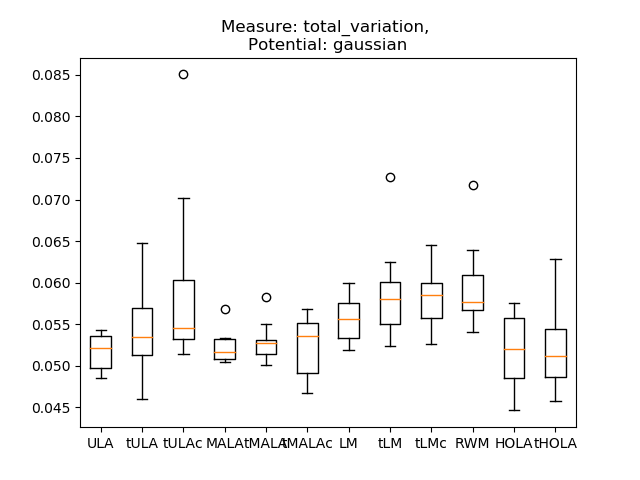
\includegraphics[height=0.43\textheight]{Figures/TV_gaussian11_step0pt02.png}
	\caption{$10^5$ samples from standard Gaussian with step size 0.02}
	\label{fig:TVgauss}
\end{figure}

\begin{figure}[ht!]
	\centering
		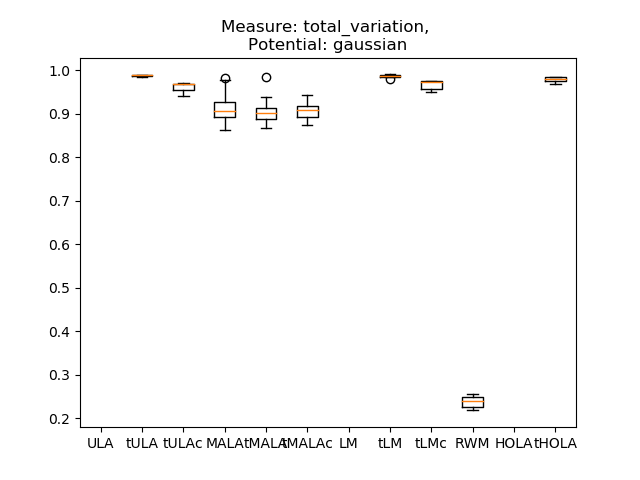
\includegraphics[height=0.43\textheight]{Figures/TV_ICgaussian10pt0001_step0pt02.png}
	\caption{$10^5$ samples from ill-conditioned Gaussian with step size 0.02}
	\label{fig:TV_ICgauss}
\end{figure}

\begin{figure}[ht!]
	\centering
		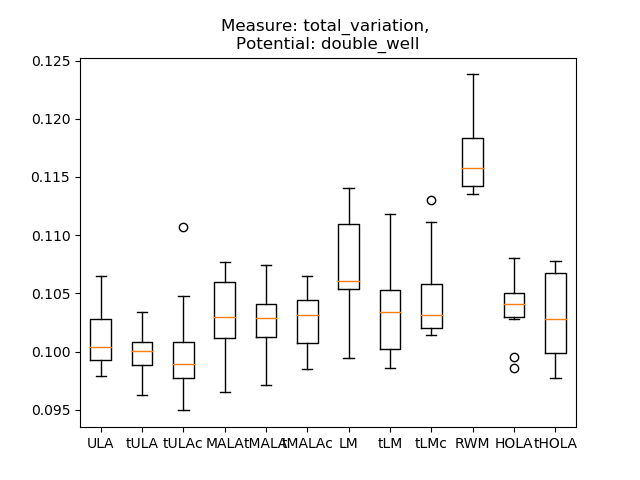
\includegraphics[height=0.43\textheight]{WriteUp/TV_doublewell_step0pt02.png}
	\caption{$10^5$ samples from double well with step size 0.02}
	\label{fig:TVdouble02}
\end{figure}

\begin{figure}[ht!]
	\centering
		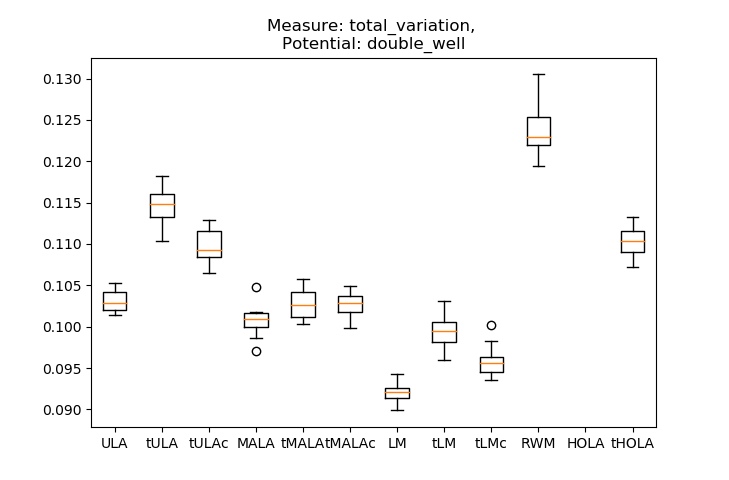
\includegraphics[height=0.43\textheight]{WriteUp/TV_doublewell_step0pt1.png}
	\caption{$10^5$ samples from double well with step size 0.1}
	\label{fig:TVdouble1}
\end{figure}

\begin{figure}[ht!]
	\centering
		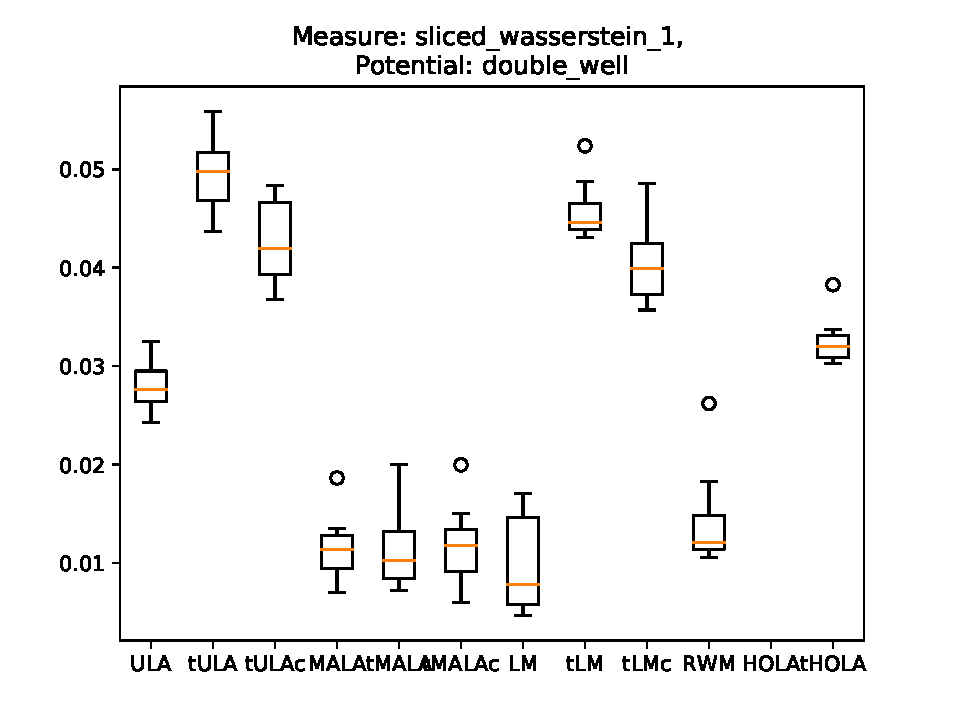
\includegraphics[height=0.43\textheight]{WriteUp/SW_doublewell_0pt1.pdf}
	\caption{SW1 distance $10^5$ samples from double well with step size 0.1}
	\label{fig:SWdouble1}
\end{figure}

\begin{figure}[ht!]
	\centering
		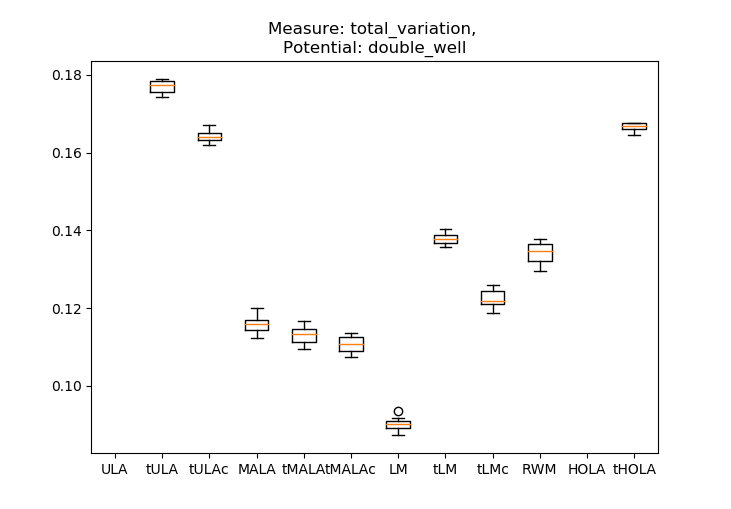
\includegraphics[height=0.43\textheight]{WriteUp/TV_doublewell_step0pt2.png}
	\caption{$10^5$ samples from double well with step size 0.2}
	\label{fig:TVdouble2}
\end{figure}

\begin{figure}[ht!]
	\centering
		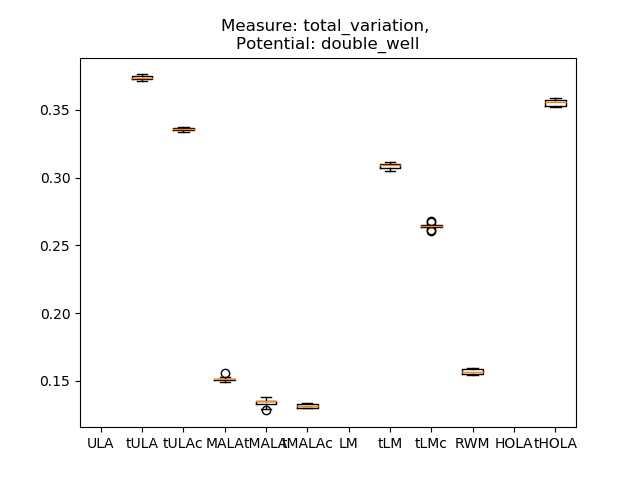
\includegraphics[height=0.43\textheight]{WriteUp/TV_doublewell_step0pt3.png}
	\caption{$10^5$ samples from double well with step size 0.3}
	\label{fig:TVdouble3}
\end{figure}

\begin{figure}[ht!]
	\centering
		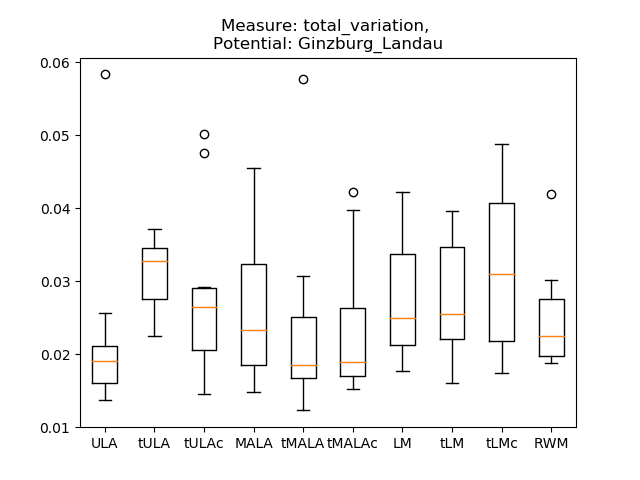
\includegraphics[height=0.43\textheight]{WriteUp/TV_ginzburg_step0pt01.png}
	\caption{$10^5$ samples from 1D Ginzburg Landau with step size 0.01}
	\label{fig:TVginz01}
\end{figure}

\begin{figure}[ht!]
	\centering
		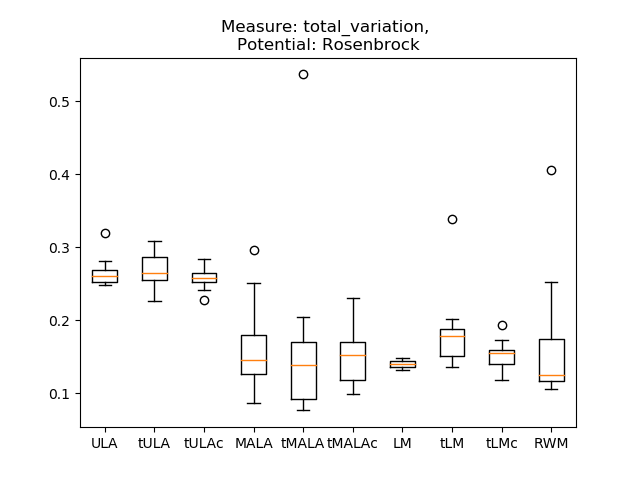
\includegraphics[height=0.43\textheight]{WriteUp/TV_rosenbrock_step0pt001.png}
	\caption{$10^5$ samples from Rosenbrock with step size 0.001}
	\label{fig:TVrosen001}
\end{figure}

\begin{figure}[ht!]
	\centering
		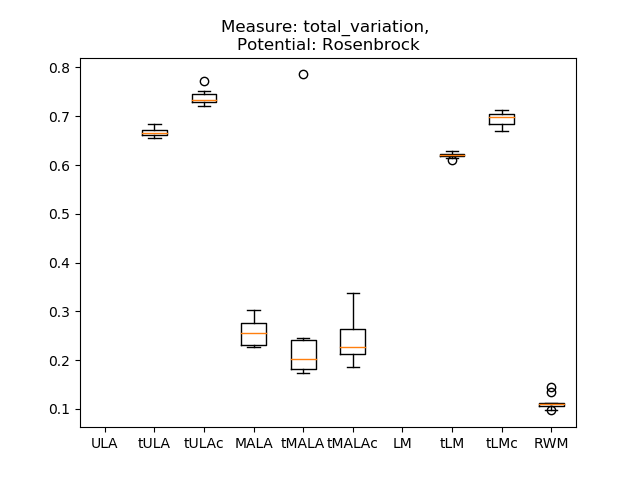
\includegraphics[height=0.43\textheight]{WriteUp/TV_rosenbrock_step0pt01.png}
	\caption{$10^5$ samples from Rosenbrock with step size 0.01}
	\label{fig:TVrosen01}
\end{figure}

\newpage
\subsection{Theoretical Non-asymptotic Error Bounds}

While the asymptotic behaviour of \texttt{ULA} and \texttt{MALA} is well-understood \cite{RT96}, the results do not consider the effect of dimension on the complexity of the algorithms.  For practical purposes, an understanding of the non-asymptotic behaviour of the algorithms would be useful and, in particular, theoretical results which could determine the step size and number of iterations required to guarantee an error of no more than some acceptable value $\epsilon$.

Theoretical bounds of this nature were first provided in \cite{dalalyan2017theoretical}, which proved bounds on the total variation distance between the distribution of the $n^{\text{th}}$ iterate of the unadjusted Langevin Algorithm, under restrictive assumptions, which will be outlined shortly.  In the case of a `warm start', where the distribution of the initial value is close to $\Pi$, it was shown that \texttt{ULA} had an upper bound of $\mathcal{O}(d/\epsilon)$ iterations to achieve precision level $\epsilon$.  This result was improved by \cite{durmus2016high, durmus2017nonasymptotic} which extended the analysis to the Wasserstein distance and dispensed with the assumption of a warm start, showing that the upper bound on iterations could be reduced to $\mathcal O (d/\epsilon)$, provided the Hessian of the potential is Lipschitz continuous.  Most recently, \cite{dalalyan2019user} has provided `user-friendly' bounds on the Wasserstein distance, further improving the constants in these bounds.

It is important to note here that these results provide explicit constants for the non-asymptotic behaviour for \texttt{ULA}.  This is in contrast to the theory for \texttt{MALA} \cite{bou2013nonasymptotic}, and the tamed \cite{Brosse18tULA} and higher order algorithms \cite{Sabanis18tHOLA}, for which only the existence of a constant is proven.  For the Leimkuhler--Matthews method, no such guarantees are known.  As such the non-asymptotic theory for the unadjusted algorithm is practically much more useful.

\subsubsection{Non-asymptotic Bounds for \texttt{ULA}}
We present without proof the results of \cite{durmus2017nonasymptotic, dalalyan2019user} which to our knowledge are the best known bounds in total variation and Wasserstein distance respectively. For both results we assume that the potential $U$ is continuously differentiable on $\R^d$, and there exist positive constants $m$ and $M$ such that $U$ is $m$-strongly convex and $M$-gradient Lipschitz, i.e. for all $x$, $y \in \R^d$,
\begin{align} \label{m-convex}
    &\text{($m$-strongly convex) \ } U(x) - U(y) - \grad U(y)^\top (x - y) \geq \frac{m}{2}\norm{x-y}_2^2\\
    &\text{($M$-gradient Lipschitz) \ } \norm{\grad U(x) - \grad U(y)}_2 \leq M \norm{x-y}_2. \label{M-GradLipschitz}
\end{align}

Denote the unique minimiser of $U$ by $y=\arg \min_{x \in \R^d} U(x)$.  Let $\nu_N$ denote the distribution of the $N^{\text{th}}$ sample

\begin{theorem}[Total Variation part (i)]
    Assume $h \in (0, 2/(m+M))$ and $U$ satisfies the assumptions (\ref{m-convex}, \ref{M-GradLipschitz}) above.  Let $\kappa = \frac{2mM}{m+M}$  Then for any initial value $x_0 \in \R^d$ and $N \geq 1$,
    $$
    \norm{\pi_h - \nu_N}_{TV} \leq \left\{ 4 \pi \kappa (1-(1-\kappa h)^{N/2} \right\}^{-1/2} (1-\kappa \gamma)^{N/2} \left\{ \norm{x_0 - y}_2 + (2 \kappa^{-1}d)^{1/2} \right\}
    $$
\end{theorem}

\begin{theorem}[Total Variation part (ii)]
    Assume $h \in (0, 1/(m+M))$, $U$ satisfies the assumptions (\ref{m-convex}, \ref{M-GradLipschitz}) above, and further, assume that $U$ is three times continuously differentiable, and there exists $L$ such that for all $x,y \in \R^d$,
    $$
    \norm{\grad^2 U(x) - \grad^2 U(y)} \leq L \norm{x-y}.
    $$
    Then
    \begin{align*}
        \norm{\pi_h - \pi}_{TV} &\leq (4 \pi)^{-1/2} \left\{ h^2 E_1(h, d) + 2dh^2 E_2(h)/(\kappa m)\right\}^{1/2}\\
        &+ (4 \pi)^{-1/2} \lceil \log(h^{-1}/\log(2) \rceil \left\{ h^2 E_1(h,d) + h^2 E_2(h)(2 \kappa^{-1}d + d/m) \right\}^{1/2}\\
        &+ 2^{-3/2} M \left\{ 2d h^3 L^2/(3\kappa) + dh^2\right\}^{1/2}
    \end{align*}
    where $E_1(h,d)$ and $E_2(h)$ are defined as
    \begin{align*}
        E_1(h,d) &= 2 d \kappa^{-1} \left\{2L^2 + 4 \kappa^{-1} (dL^2/3 + h M^4 /4) + h^2 M^4/6 \right\}\\
        E_2(h) &= L^4(4\kappa^{-1}/3 + h)
    \end{align*}
\end{theorem}

The triangle inequality gives our desired bound on $\norm{\pi - \nu_N}_{TV}$.  We next present the `user-friendly' bound in Wasserstein distance.

\begin{theorem}[Wasserstein distance]
    Assume $h \in (0, 2/M)$ and $U$ satisfies the assumptions (\ref{m-convex}, \ref{M-GradLipschitz}) above. 
    \begin{itemize}
        \item If $h \leq \frac{2}{m+M}$, then $W_2(\nu_N, \pi) \leq (1-mh)^N W_2(\nu_0, \pi) + 1.65 \frac{M}{m}(hp)^{1/2}.$
        \item If $h \geq \frac{2}{m+M}$, then $W_2(\nu_N, \pi) \leq (Mh-1)^N W_2(\nu_0, \pi) + \frac{1.65Mh}{2-Mh}(hp)^{1/2}.$
\end{itemize}
\end{theorem}
\begin{prop}
    If the initial value $X_0 = x_0$ is deterministic then,
    $$
    W_2(\nu_0, \pi)^2 = \int_{\R^p} \norm{x_0-x}_2^2 \pi(dx) \leq \norm{x_0-y}_2^2 + \frac{p}{m}.
    $$
\end{prop}

\begin{remark}
    If we choose $h$ and $N$ such that
    $$
    h \leq \frac{2}{m+M}, \quad e^{-mhN}W_2(\nu_0, \pi) \leq \epsilon/2, \quad 1.65\frac{M}{m}(hp)^{1/2} \leq \epsilon/2
    $$
    then $W_2(\nu_N,\pi) \leq \epsilon$.  Hence, for a deterministic initial value $X_0=x_0$, it is sufficient to choose
    $$
    h \leq \frac{m^2 \epsilon^2}{11M^2p} \wedge \frac{2}{m+M}, \quad hN \geq \frac{1}{m} \log \left( \frac{2(\norm{x_0-y}_2^2+p/m)^{1/2}}{\epsilon} \right)
    $$
    for a precision $\epsilon$ in $W_2(\nu_K, \pi)$.
\end{remark}

\begin{note}
    In practice, $\norm{x_0-y}_2$ may be difficult to calculate.  An alternative bound can easily be derived from the strong convexity of $U$ and the fact that $y$ minimises $U$:
    \begin{align*}
        m W_2(\nu_0, \pi)^2 &\leq m \norm{x_0-y}_2^2 + p\\
        &\leq 2(f(x_0) - f(y) - \nabla U(y)^{\top}(x_0-y) + p\\
        &= 2(f(x_0)-f(y))+p.
    \end{align*}
    If $U$ is bounded below by a constant, say $U \geq 0$, this provides an easily computable upper bound on $W_2(\nu_0, \pi)$.
\end{note}

\subsubsection{Numerical Tests}
